\documentclass[10pt,twocolumn]{article}
\usepackage[T1]{fontenc}
\usepackage[utf8]{inputenc}
\usepackage{lmodern}
\usepackage{microtype}
\usepackage[margin=0.75in,columnsep=0.25in]{geometry}
\usepackage{booktabs}
\usepackage{graphicx}
\usepackage{amsmath}
\usepackage[numbers,sort&compress]{natbib}
\usepackage[hidelinks]{hyperref}
\usepackage{xcolor}
\usepackage{enumitem}
\setlist{nosep,leftmargin=1.1em}
\setlength{\tabcolsep}{3.2pt}
\newcommand{\pend}[1]{\textcolor{gray}{\emph{[pending: #1]}}}

\title{\textbf{KVKK-Bench: Measuring Personal-Data Masking in Turkish Legal Text,\\with Small On-Device Models}}
\author{Fikri F{\i}rat\\{\small Katip \,\textperiodcentered\, \url{https://github.com/fikrifirat/katip}}}
\date{Draft, 14 November 2026}

\begin{document}
\maketitle

\begin{abstract}
Turkish lawyers increasingly paste client documents into general-purpose AI assistants. The Turkish
data-protection authority's 2026 guide for lawyers states that this can amount to a transfer of personal data
abroad under art.~9 of Law No.~6698 (KVKK), and recommends masking personal data first. Masking needs a detector
that works on Turkish legal prose and can run on the lawyer's own machine, but published Turkish PII models are
evaluated on their own, mostly synthetic, data. We release \textbf{KVKK-Bench}, a public benchmark with a fixed
scorer that ranks systems on real text only (Yarg{\i}tay sentences with held-out Turkish and foreign names, and
Wikipedia sentences), reports a character-level \emph{leak rate}, and closes a loophole by which over-masking
scored perfect precision. We evaluate 14 systems and release two small models, \textbf{Katip Mask Base}
(110M parameters, 111\,MB int8) and \textbf{Katip Mask Nano} (2.5M, 2.9\,MB, 50 pages/s on a laptop CPU), both of
which run in a browser. Base scores 97.0 Overall [95\% CI 96.5--97.5], 1.1 points above the best general model
(XLM-R Large, 95.9) but with twice its leak rate (6.9\% vs 3.4\%). We do not claim a state of the art: the
margins are small, part of the test is in-domain for our models, and no real client documents are labelled yet.
The contribution is a shared, reproducible yardstick and a practical model family for local masking.
\end{abstract}

\section{Motivation}
\label{sec:motivation}

\textbf{Legal setting.} Law No.~6698 (KVKK) governs personal data in T{\"u}rkiye \citep{kvkk6698}. Since 1 June
2024, transfers abroad follow a GDPR-like tiered regime (adequacy decision, then appropriate safeguards such as
standard contracts notified to the Authority, then narrow incidental exceptions; art.~9 as amended by Law
No.~7499) with implementing rules in a July 2024 regulation \citep{kvkk-transfer-reg}. In September 2026 the
Authority published an application guide for lawyers, prepared with the Union of Turkish Bar Associations
\citep{kvkk-lawyers-guide}. It treats lawyers as data controllers, notes that their exemption from the
controllers' registry (Board decision 2018/32 \citep{kvkk-2018-32}) does not exempt them from other duties, and
has a section on generative AI. It names ChatGPT, Claude and Gemini and states that uploading client files or
case documents containing personal data may constitute a transfer abroad under art.~9 when the provider, its
servers or its sub-processors are abroad, and a domestic transfer under art.~8 otherwise (pp.~120--121). It
recommends masking or anonymising personal data ``as far as possible'', not uploading special-category data,
and sharing only the minimum needed (p.~146).

\textbf{Enforcement.} The guide quotes Board decisions that fined lawyers for unlawful processing, e.g.\ 2020/429
(phone numbers of a debtor's relatives and colleagues) \citep{kvkk-2020-429}, 2021/111 (50,000~TL, an SMS to a
number known to belong to a relative) \citep{kvkk-2021-111} and 2021/1111 (a witness's criminal record obtained
without authority and used in a petition) \citep{kvkk-2021-1111}. It also quotes decisions finding no violation
where a lawyer submitted personal or special-category data to a court for the client's case (2021/925, 2023/1414)
\citep{kvkk-2021-925,kvkk-2023-1414}. So the exposure is not court filing as such; it is sending client data to
third parties without a legal basis, which is what pasting a file into a foreign AI service can be.

\textbf{Why on-device.} A remote masking service, or a connector run by the AI provider, moves the original
document off the lawyer's machine before anything is masked. Only masking on the device keeps the originals
local. That requires a detector that is (i) accurate on real Turkish legal prose, with court casing
(\emph{Ahmet YILMAZ}), case suffixes (\emph{Kaya'n{\i}n}) and foreign clients' transliterated names, and
(ii) small enough for a browser tab or a laptop. Masked text is still pseudonymised personal data, so masking
reduces but does not remove KVKK obligations.

\textbf{Gap.} Several Turkish PII models are public, but each reports on its own data, usually synthetic or a
validation split. Our own first model illustrates the risk: BERTurk fine-tuned on synthetic legal documents found
every name in synthetic tests and 41\% of names in real Wikipedia sentences \citep{katip-repo}. Existing
anonymisation benchmarks are English (TAB, ECHR cases \citep{pilan2022tab}; i2b2 clinical notes
\citep{stubbs2015i2b2}). Turkish legal NER data exists \citep{cetindag2022tlner} but its person names are mostly
anonymised as ``\ldots''.

\section{KVKK-Bench}
\label{sec:bench}

\textbf{Real-text tracks (ranked).} \emph{court-turkish}: the 109 sentences of the TurkishLegalNER \emph{test}
split \citep{cetindag2022tlner} that contain anonymised person slots, each slot filled three times (327 documents,
20,346 words, 1,011 names). Names come from Wikidata (CC0): given and family names of Turkish citizens, kept only if
no word of the name appears in Katip's lexicons, any synthetic training set or Turkish Wiki NER train, so no
system can score by memorising them. Casing follows court style (Title 43\%, \emph{Ahmet YILMAZ} 37\%, all caps
20\%) and the case suffix after each slot is re-inflected to agree with the new name. \emph{court-foreign}: the
same slots filled with names from held-out families of nine origin groups (Arab, Persian, Afghan, Georgian,
Armenian, Greek, Slavic, Azerbaijani, Western) with real-world transliteration variants (327 documents, 1,011
names); the two court tracks are paired by slot. \emph{prose}: the 1,000 sentences of the Turkish Wiki NER test
split, PERSON spans only, as annotated by its authors \citep{altinok2023} (654 names).

\textbf{Generated tracks (check only).} Petitions, contracts, correspondence, health records and court filings
from Katip's generator (80 documents, 16 styles, seed 4242) and 300 generated petitions about foreign clients with
foreigner IDs (YKN), passports and home-country IDs. They carry every non-name type (TCKN, VKN, IBAN, phone,
e-mail, address, plate, birth date, health). Because Katip's models are trained on the same generator family
(with different names), these tracks are shown as a regression check and are \emph{excluded} from the ranking.
A name-free legal-prose track (3 documents) counts false alarms.

\textbf{Scorer.} A gold value is \emph{found} if a predicted span of the same type covers it, or lies inside it
and covers at least half of it (and $\geq$3 characters; whitespace- and case-insensitive). A predicted span is
\emph{correct} if it overlaps a gold value of its type \emph{and} at least half of its letters and digits lie
inside such values. The second condition is a fix in v0.1.2: before it, one span over the whole document scored
100\% precision. Per dimension we compute F2 \citep{vanrijsbergen1979} from pooled recall and precision (a miss
costs four times a false alarm). \textbf{Overall} is the weighted mean of three real-text name dimensions:
Turkish names in court text (weight 25), foreign names in court text (10), names in general prose (10). The
\textbf{leak rate} is the share of gold personal-data characters left unmasked by any predicted span, averaged
over the three real tracks; a half-masked name counts as half a leak. We also report the clean-document rate and
false alarms per 1,000 words.

\textbf{Uncertainty.} 95\% CIs come from a percentile bootstrap \citep{efron1993} with 10,000 resamples that
resamples the 109 court sentences as clusters (keeping their three fills and both court tracks together) and the
1,000 prose sentences independently. Comparisons with Katip Mask Base are paired (same resample for both systems);
we report two-sided bootstrap $p$-values and correct across the 13 comparisons with Holm's method \citep{holm1979}.

\textbf{Release.} Public split, scorer, runner, saved predictions of every system and the leaderboard Space are
open \citep{firat2026kvkkbench,katip-repo}; a canary string marks every file. Licences follow the sources:
TurkishLegalNER annotations Apache-2.0 (court decisions carry no copyright under FSEK art.~31), Wiki NER
CC BY-SA 4.0, generated documents CC BY 4.0. Every inserted value is synthetic.

\section{Systems}
\label{sec:systems}

\textbf{Katip Mask Base · tr v2}: BERTurk \citep{schweter2020berturk} fine-tuned for 3 epochs on 8,000 synthetic
legal documents plus 17,967 Turkish Wiki NER \emph{train} sentences (person names), tagging names, addresses and
health terms; int8 ONNX. \textbf{Katip Mask Nano · tr v1.1}: a 2-layer BERT (hidden 128, 16k WordPiece) trained from
scratch for 5 epochs (458\,s on 4 CPU cores) on 8,000 synthetic documents, 4,182 real-text documents (Wiki NER
train, TurkishLegalNER \emph{train}-split sentences with filled names) and a transliterated foreign-name mix whose
test families were held out. Both run inside Katip's rule engine (checksummed IDs, phones, IBANs, addresses,
casing and suffix handling; 0.3\,MB) with the browser's own code at a confidence threshold of 0.5 chosen on dev
data. \textbf{Baselines} (run unmodified, label maps written from each model's \texttt{id2label} before scoring):
Presidio with spaCy \texttt{xx\_ent\_wiki\_sm} \citep{presidio}; Turkish NER (BERTurk NER, XLM-R Base Turkish NER);
XLM-R Large fine-tuned on English CoNLL-03 \citep{conneau2020xlmr}; GLiNER multi-PII \citep{zaratiana2024gliner}
and GLiNER2 PII \citep{zaratiana2025gliner2} prompted with \emph{person}; Turkish PII models (ModernBERT-TR PII,
OpenMed PII Turkish 33M); multilingual PII models (OpenAI Privacy Filter \citep{openai-pf}, OpenMed Privacy Filter
v2, Piiranha); and Qwen2.5-1.5B-Instruct \citep{qwen2025} prompted to list personal data as JSON. All systems
receive identical text and are timed on one Apple-silicon laptop (12 CPUs) in Python; a page is 500 words.

\section{Results}
\label{sec:results}

\begin{table*}[t]
\centering\footnotesize
\setlength{\tabcolsep}{2.6pt}
\begin{tabular}{@{}lrrrrrrrrr@{}}
\toprule
System & Params & Size MB & Pages/s & \textbf{Overall} [95\% CI] & TR names & Foreign & Prose & Leak \% [95\% CI] & Browser \\
\midrule
\textbf{Katip Mask Base} (ours) & 110M & 111 & 1.7 & \textbf{97.0} [96.5, 97.5] & \textbf{98.6} & 96.3 & 88.9 & 6.9 [5.9, 8.1] & yes \\
XLM-R Large (CoNLL-en) & 559M & 2,235 & 2.3 & 95.9 [94.9, 96.7] & 97.6 & 97.5 & \textbf{89.9} & \textbf{3.4} [2.9, 3.9] & -- \\
XLM-R Base Turkish NER & 277M & 1,110 & 5.7 & 95.7 [94.8, 96.6] & 98.5 & \textbf{98.2} & 86.3 & 6.6 [5.6, 7.8] & -- \\
GLiNER2 PII (person) & 307M & 1,228 & 1.2 & 95.0 [94.1, 95.8] & 98.1 & \textbf{98.2} & 83.9 & 5.8 [4.8, 7.0] & -- \\
BERTurk NER & 110M & 440 & 6.0 & 91.6 [88.8, 93.4] & 97.4 & 91.7 & 77.1 & 8.1 [6.9, 9.4] & -- \\
GLiNER multi PII & 289M & 1,156 & 1.1 & 91.3 [85.7, 95.5] & 93.1 & 92.9 & 85.2 & 10.5 [5.6, 16.7] & -- \\
\textbf{Katip Mask Nano} (ours) & 2.5M & \textbf{2.9} & \textbf{50.0} & 86.3 [84.8, 87.7] & 93.3 & 93.1 & 57.8 & 18.5 [16.7, 20.4] & yes \\
ModernBERT-TR PII & 149M & 598 & 4.8 & 85.3 [83.9, 86.6] & 98.5 & 96.5 & 39.1 & 21.6 [19.7, 23.6] & -- \\
Qwen2.5-1.5B, prompted & 1.5B & 3,087 & 0.01 & 57.5 [46.2, 68.1] & 56.7 & 55.1 & 47.6 & 41.1 [31.3, 52.1] & -- \\
OpenMed Privacy Filter v2 & 1.4B & 2,799 & 0.17 & 57.2 [55.4, 59.1] & 57.0 & 54.7 & 48.3 & 36.4 [34.2, 38.2] & -- \\
OpenAI Privacy Filter & 1.4B & 2,799 & 0.11 & 51.3 [44.7, 56.2] & 57.0 & 57.2 & 27.6 & 52.5 [48.1, 58.3] & -- \\
Piiranha v1 & 278M & 1,113 & 2.9 & 49.8 [45.4, 55.7] & 40.8 & 60.2 & 56.7 & 45.4 [40.0, 49.4] & -- \\
Presidio + spaCy xx (baseline) & -- & 11 & 31.3 & 45.0 [42.1, 47.7] & 38.9 & 43.6 & 60.4 & 31.7 [29.8, 33.4] & -- \\
OpenMed PII Turkish 33M & 33M & 133 & 7.5 & 19.1 [16.4, 22.7] & 11.0 & 17.3 & 33.4 & 73.0 [69.8, 75.6] & -- \\
\bottomrule
\end{tabular}
\caption{KVKK-Bench v0.1.2, public split, real-text tracks. Overall and the three name columns are F2 (\%); the
name columns are per-track F2 (court-turkish, court-foreign, prose). Leak = share of gold characters left
readable (lower is better). CIs: sentence-clustered bootstrap, 10,000 resamples. Size = what is downloaded to run
(int8 ONNX plus rules for Katip; weights as loaded otherwise). Pages/s: Python on one Apple-silicon laptop; not an
in-browser speed. Browser = run inside a web page via transformers.js/ONNX Runtime Web (not tested is not
impossible). Numbers match the live leaderboard and the saved predictions.}
\label{tab:main}
\end{table*}

\textbf{Main result (Table~\ref{tab:main}).} Katip Mask Base has the highest Overall, 97.0. Its lead over XLM-R
Large is 1.1 points [0.3, 2.1], over XLM-R Base Turkish NER 1.3 [0.5, 2.2] and over GLiNER2 2.1 [1.2, 3.0]; all
13 paired differences remain significant after Holm correction (largest adjusted $p=0.008$). These margins are
small, and the ranking depends on the metric: XLM-R Large leaks \emph{half as much} (3.4\% vs 6.9\%, difference
3.5 points [2.5, 4.6]); the leak difference with XLM-R Base, GLiNER2, BERTurk NER and GLiNER is not significant
(all $p>0.1$). Base is the best system that runs in a browser, at one twentieth of XLM-R Large's download size.

\textbf{Small models.} Nano reaches 93.3/93.1 F2 on Turkish and foreign names in court text at 2.9\,MB and
50 pages/s, 29 times faster than Base, but collapses on general prose (57.8 F2, 44.5\% leak): a sub-5\,MB model
covers legal register, not open-domain Turkish. Off-the-shelf multilingual PII models of 1.4B parameters score
51--57, below the 11\,MB Presidio on prose and far below Turkish NER models on court text; a prompted 1.5B LLM is
both slow (80\,s per page on CPU) and unreliable (57.5, CI width 22 points).

\textbf{Error analysis (Base).} On court-turkish it misses 1 of 1,011 names; its 5 false spans are rapporteur
names whose span also swallowed the title (\emph{Tetkik Hakimi \ldots}), so the name is masked but the span fails
the 50\% rule. On court-foreign it misses 30 of 1,011; recall by origin is 95--100\% except Azerbaijani names
(82\%, 41/50), which are often built from Turkish word stems (XLM-R Large: 98\%). On prose it misses 67 of 654:
single-token names 11\% (32/300) and names of three or more tokens 27\% (22/81), versus 5\% for two-token names;
false spans are mostly titles of works and organisations (\emph{Bohemian Rhapsody}, \emph{Florya Metin Oktay}).
The higher leak rate of Base versus XLM-R Large comes from prose (17.6\% vs 9.8\%), i.e.\ long and single-token names
in open-domain text. XLM-R Large's false spans are mostly lone punctuation tagged PER (harmless for privacy).

\begin{figure}[t]
\centering
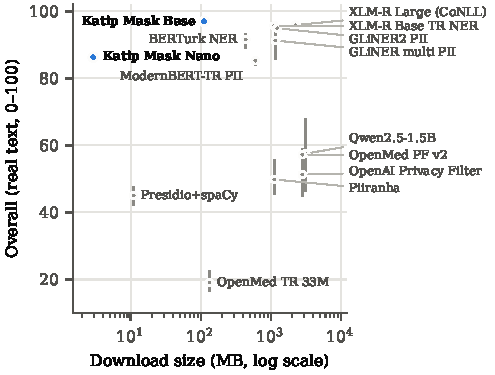
\includegraphics[width=\columnwidth]{fig_overall_size.pdf}
\caption{Overall (95\% CI) against download size. Blue: Katip Mask models, both run in a browser.}
\label{fig:size}
\end{figure}

\textbf{Generated tracks (not ranked).} With Katip's rules, Base and Nano find every TCKN, phone, e-mail and
address in the generated documents, and Base finds 95.7 F2 of health terms. Name-only systems score 0 on these
types by construction. One harness defect surfaced while writing: the benchmark run used a rule file without the
YKN, passport and foreign-ID recognisers shipped in the app, so both Katip rows score 0 on those 557 values
(``Other IDs'' 16.5). Re-running the shipped rules alone on that track finds 100\% of YKN and passports and 96\% of
foreign IDs; the leaderboard rows will be re-run \pend{bench re-run with current rules}.

\section{Distribution: local masking in front of AI assistants}
Katip Mask runs as a static web page (rules in Python via Pyodide, models via transformers.js) and as
\textbf{Katip Kalkan}, a local MCP server packaged as a Claude plugin
(\texttt{claude plugin marketplace add fikrifirat/katip}). Kalkan masks a file on the device with Nano, gives the
assistant only the masked text, and writes real values back into the assistant's answer locally, so originals
never reach the AI provider. It also runs local OCR (PaddleOCR via ONNX) for scans and photos.

\section{Limitations and future work}
\begin{itemize}
\item \textbf{No real client documents.} Court sentences with filled slots and Wikipedia are proxies. Contracts,
petitions and e-mails from practice are the target of a consented pilot whose documents never leave the firm;
private lawyer documents are not and will not be in the benchmark.
\item \textbf{Names only on real text.} IDs, addresses and health data appear only in generated documents from
the generator family our models train on, so every non-name figure above is optimistic and excluded from Overall.
\item \textbf{In-domain advantage.} The prose track is the Wiki NER test split; Base and Nano were trained on its
train split, and Nano on TurkishLegalNER's train split (the court tracks use its test split). Other models were
trained on their own Turkish or multilingual NER data. A hidden test of 2025--26 Yarg{\i}tay/Dan{\i}{\c{s}}tay decisions
and AYM judgments with court-published names is under construction \pend{hidden split}.
\item \textbf{Slot filling} puts names where courts wrote ``\ldots'', which a model could learn to exploit; the AYM
real-name track is meant to check this.
\item \textbf{One annotator}; inter-annotator agreement on 100 hidden documents is planned \pend{Cohen's $\kappa$}.
\item \textbf{Speed} is measured in Python on one laptop. ``Runs in the browser'' means demonstrated, not timed.
\item \textbf{OCR} is tested only on Katip's own scans and synthetic phone photos. Adding OCRTurk
\citep{ocrturk2026} as an OCR track awaits a licence from its authors \pend{licence}.
\item \textbf{Licences.} Both models are CC BY-SA 4.0 because they are trained on Wiki NER; code is AGPL-3.0. A v3
retrained without Wikipedia data (synthetic, court decisions, TurkishLegalNER) would allow Apache-2.0, if it stays
within about one Overall point \pend{v3}. Fine-tuning XLM-R on our data is running \pend{XLM-R fine-tune}.
\item \textbf{Masking is not anonymisation.} Masked documents remain personal data under KVKK; the tool reduces
exposure but does not by itself make an AI workflow compliant.
\end{itemize}

\textbf{Reproducibility.} \texttt{lab/legal/bench\_build.py} rebuilds the public split from public sources;
\texttt{bench\_run.py --rescore} re-scores the saved predictions; the CI script and figure are in
\texttt{paper/}. All numbers in this draft were reproduced from those files on 14 November 2026.

\small
\bibliographystyle{plainnat}
\bibliography{refs}

\end{document}
